\documentclass[12pt]{article}
\title{\textbf{TELLIE PCA: \\ Processing automation}}
\date{February 2023}
\author{Michal Rigan}
\usepackage{hyperref}
\hypersetup{
     colorlinks   = true,
     urlcolor = blue,
     citecolor    = grey
}
\hypersetup{colorlinks=true}
\usepackage{graphicx}
\usepackage{listings}
\lstset{
    basicstyle=\ttfamily\footnotesize,
    frame=single, % adds a frame around the code
    xleftmargin=3.4pt,
    xrightmargin=3.4pt,
}
\graphicspath{ {images/} }
\begin{document}

\maketitle{}

\vspace{7cm}
\paragraph{}
This document describes what the TELLIE PCA automation does, why, and how.
\clearpage

\section{Content}
\paragraph{}
\begin{itemize}
	\item Why automation
	\item Overview
	\item Data-taking
	\begin{itemize}
		\item Validation \#1
	\end{itemize}
	\item Data-processing
	\begin{itemize}
		\item PCA table generation
		\begin{itemize}
			\item Beamspot fit
			\item Direction fit
			\item Angular systematic
			\item Injection time fit
		\end{itemize}
		\item Validation \#2
		\item PCA constants
		\item Benchmarking
		\item Monitoring
	\end{itemize}
	\item Code %mention checks, structure
	\item Deploying %(mention requirements here: rat, python, dbs...)
	\item Running
	\item ToDos
	\item Other documentation %tellie guides (2), PCA guide, my thesis
\end{itemize}

\section{Why automation}
\paragraph{}
The process of extracting and validating PCA constants from TELLIE data is complex. This piece of software was developed to streamline the process of obtaining the PCA constants, at reasonably high speed. \\
Additionally, it was designed to:
\begin{itemize}
	\item be independent of the method used for Data-taking
	\item be modular, easily modifiable and configurable
	\item require minimal human input
	\item provide monitoring
	\item be mostly standalone
\end{itemize}

\section{Overview}
\paragraph{}
The TELLIE PCA Automation overview is shown in Figure~\ref{fig:overview}.\\There are two main parts: TELLIE \textbf{\texttt{Data-taking}} and \textbf{\texttt{Data-processing}}.

\paragraph{}
Data-taking is done independently of the processing (as the exact method was not yet finalised before developing processing). More information can be found in \href{https://www.snolab.ca/snoplus/private/DocDB/cgi/ShowDocument?docid=7612}{TELLIE Data-taking automation document}. It should be noted that \texttt{Validation \#1} is taken care of by Data-processing.

\paragraph{}
Data-processing is everything that is done with TELLIE PCA data once it is stored. This includes performing checks on the data, making fits required for further processing, generating tables (both local and online), extracting PCA constants, benchmarking these constants, and a suite of monitoring for these steps. These will be described below.

\begin{figure}
\centering
\noindent\makebox[1\textwidth]{
  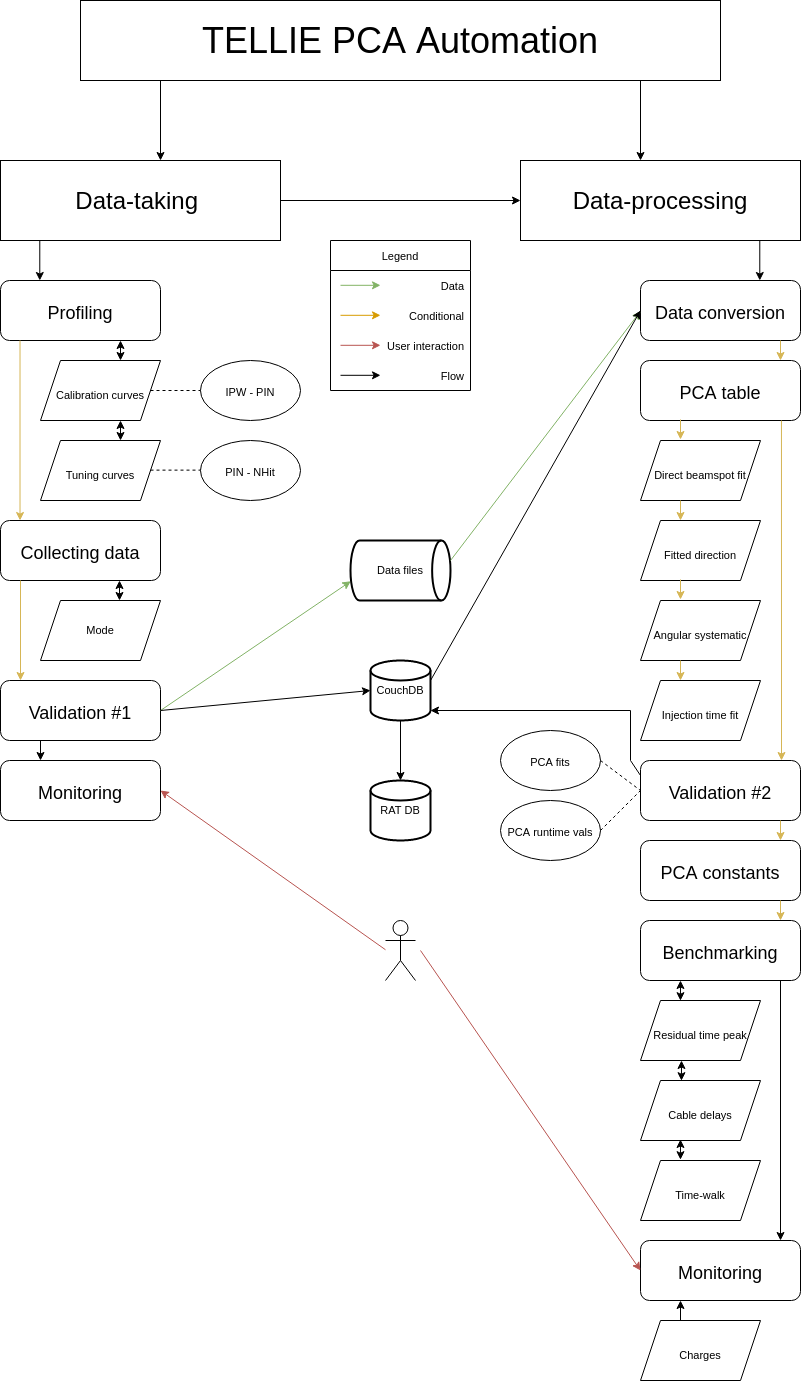
\includegraphics[width=0.9\textwidth]{./plots/overview.png}}
  \caption{\centering Overview of the TELLIE PCA Automation.}
  \label{fig:overview}
\end{figure}

\section{Data-taking}
\subsection{Validation \#1}
\paragraph{}
As mentioned above, even though \texttt{Validation \#1} is logistically part of Data-taking, it is performed by Data-processing, and is also independent of the method the data was taken.\\
\textbf{Goal:} Validate that the data is of required quality for PCA.

%where in code
%what checks
%page
%plots

\section{Data-processing}
\subsection{PCA table generation}
\paragraph{}
There are several corrections that need to be fitted for, which are later used for the extraction of PCA constants. The fits need to happen in succession, as the output of one feeds into the next. Between steps, these are stored as text files. After all fits are made, a local table is produced, combining the corrections. This table is loaded by the PCA Processor.\\
\textbf{Goal:} Make fits, obtain corrections required for the extraction of PCA constants. Produce final PCA table.

\subsubsection{Fit: beamspot}

\subsubsection{Fit: direction}

\subsubsection{Fit: angular systematic}

\subsubsection{Fit: Injection time}

\subsection{Validation \#2}
\textbf{Goal:} Check and confirm that the fits are sensible.

%where do we compare pca tables? add

\subsection{PCA constants}
\textbf{Goal:} Run the PCA Processor that extract the pca constants (both timing and charge).

\subsection{Benchmarking}
\textbf{Goal:} Compare the set of constants against the closest (previous) set. Useful to see overall stability and for highlighting outliers.

\subsection{Monitoring}
\textbf{Goal:} Provide monitoring of each step of the chain. Also compares fibres between datasets.

\section{Deploying}

\section{Running}

\section{ToDos}

\section{Other documentation}


\end{document}
